% This is based on "sig-alternate.tex" V1.9 April 2009
% This file should be compiled with V2.4 of "sig-alternate.cls" April 2009
%
\documentclass{report}

\usepackage[english]{babel}
\usepackage{graphicx}
\usepackage{tabularx}
\usepackage{subfigure}
\usepackage{enumitem}
\usepackage{url}
\usepackage{float}

\usepackage{color}
\definecolor{orange}{rgb}{1,0.5,0}
\definecolor{lightgray}{rgb}{.9,.9,.9}
\definecolor{java_keyword}{rgb}{0.37, 0.08, 0.25}
\definecolor{java_string}{rgb}{0.06, 0.10, 0.98}
\definecolor{java_comment}{rgb}{0.12, 0.38, 0.18}
\definecolor{java_doc}{rgb}{0.25,0.35,0.75}

% code listings

\usepackage{listings}
\lstloadlanguages{Java}
\lstset{
	language=Java,
	basicstyle=\scriptsize\ttfamily,
	backgroundcolor=\color{lightgray},
	keywordstyle=\color{java_keyword}\bfseries,
	stringstyle=\color{java_string},
	commentstyle=\color{java_comment},
	morecomment=[s][\color{java_doc}]{/**}{*/},
	tabsize=2,
	showtabs=false,
	extendedchars=true,
	showstringspaces=false,
	showspaces=false,
	breaklines=true,
	numbers=left,
	numberstyle=\tiny,
	numbersep=6pt,
	xleftmargin=3pt,
	xrightmargin=3pt,
	framexleftmargin=3pt,
	framexrightmargin=3pt,
	captionpos=b
}

% Disable single lines at the start of a paragraph (Schusterjungen)

\clubpenalty = 10000

% Disable single lines at the end of a paragraph (Hurenkinder)

\widowpenalty = 10000
\displaywidowpenalty = 10000

% allows for colored, easy-to-find todos

\newcommand{\todo}[1]{\textsf{\textbf{\textcolor{orange}{[[#1]]}}}}

% consistent references: use these instead of \label and \ref

\newcommand{\lsec}[1]{\label{sec:#1}}
\newcommand{\lssec}[1]{\label{ssec:#1}}
\newcommand{\lfig}[1]{\label{fig:#1}}
\newcommand{\ltab}[1]{\label{tab:#1}}
\newcommand{\rsec}[1]{Section~\ref{sec:#1}}
\newcommand{\rssec}[1]{Section~\ref{ssec:#1}}
\newcommand{\rfig}[1]{Figure~\ref{fig:#1}}
\newcommand{\rtab}[1]{Table~\ref{tab:#1}}
\newcommand{\rlst}[1]{Listing~\ref{#1}}

% General information

\title{Kompose - A distributed playlist}
\subtitle{subtitle}

% Use the \alignauthor commands to handle the names
% and affiliations for an 'aesthetic maximum' of six authors.

\numberofauthors{2} %  in this sample file, there are a *total*
% of EIGHT authors. SIX appear on the 'first-page' (for formatting
% reasons) and the remaining two appear in the \additionalauthors section.
%
\author{
% You can go ahead and credit any number of authors here,
% e.g. one 'row of three' or two rows (consisting of one row of three
% and a second row of one, two or three).
%
% The command \alignauthor (no curly braces needed) should
% precede each author name, affiliation/snail-mail address and
% e-mail address. Additionally, tag each line of
% affiliation/address with \affaddr, and tag the
% e-mail address with \email.
%
% 1st. author
    \alignauthor \normalsize{Mark Arnold (15-917-701), Dino Bollinger (14-923-676), Tobias Brodmann (15-934-565), Lino Lendi (11-714-383), Florian Moser (15-930-704), Lukas Tobler (14-942-007)}\\
	% \affaddr{\normalsize{ETH ID-1 15-917-701, ETH ID-2 14-923-676, ETH ID-3 15-934-565, ETH ID-4 11-714-383, ETH ID-5 15-930-704, ETH ID-6 14-942-007}}\\
	\email{\normalsize{arnomark@student.ethz.ch, bdino@student.ethz.ch, brotobia@student.ethz.ch, llendi@student.ethz.ch, moserfl@studen.ethz.ch, lutobler@student.ethz.ch}}
}

\begin{document}

\maketitle

\begin{abstract}
\emph{Kompose} is an Android app that allows many participants to share a playlist and
request songs to be played at social events. Users will be able to share,
synchronize and vote on YouTube songs in a fully distributed fashion. One device will
act as the host which controls the music station and plays the songs in the play queue
with the order agreed upon by all clients.
\end{abstract}

\section{Introduction}
At social events, such as parties, we often face the problem of deciding who is
in charge of the music being played. In our experience, many people will be
dissatisfied with that persons taste in music, and he will frequently be
bothered with song requests.

\emph{Kompose} solves this problem by creating a distributed playlist that anyone
can add songs to. One device will start a session (the \emph{host}, usually connected
to a stereo), and other devices on the local network can join in and start
adding songs to the queue.  Apart from choosing the name for the party,
the host will have the same functionality and capabilities as the other clients.
Clients can \emph{downvote} a specific song, and when the host realizes
a majority of clients downvoted a song, it will be removed from the play queue.  
Past sessions will be kept, so the users can review playlists at a later date.

The source of music will be YouTube. Clients send a YouTube URL with
their song request to the host. The host will then download and cache the
audio from YouTube ahead of time to allow continuous playback.

The challenges in this project are automatically announcing and finding
services on the network, synchronizing the playlist state to all devices,
and keeping track of all clients that are still alive (to allow the majority based voting). 
Adding new songs to the playlist, and voting on skipping songs should be fair 
for all clients. A protocol that supports all these features must be devised.

\section{System Overview}
\subsection{Client/Server architecture}
The host device will act as the server in our system. All communication is
done over the host, i.e. there is no peer-to-peer communication between
clients. Our communication protocol will provide functionality such as:
registering a client, unregistering a client, sending a song request,
voting to skip a song, and sending the playlist state (including all songs
in the play queue, at the received downvotes for each of the songs) to the clients.
To add some resilience against clients dropping off the network,
clients send a keep-alive message to the host every few seconds.

Both client and server listen on the network for messages,
the host for requests from the clients, and the clients for state updates
from the host. To avoid manual IP/port configuration, \emph{Network Service Discovery}
\cite{nsd} is used. This gives the clients the hosts' IP and port,
to which they can send a \emph{register} messgage containing the IP and port they
will be listening on for state updates.

For messaging, a JSON based protocol will be used over TCP.

\subsection{User interface}
Figure 1 shows a mockup of the user interface design. The start screen
(top center) allows the user to either join or create a party. The host chooses
a party name, while the clients will listen for a service announcement
from a host. If an announcement is received, the party name shows up
in a list and can be joined.

The playlist view has a list of all items currently in the play queue.
Every list item has a button to downvote.

Past playlist are available from the home screen, or from the action bar
overflow menu in the playlist view, which also has an option to leave a party.

The host will additionally have a play/pause button in the action bar.

\subsection{YouTube file downloads}
The host fetches songs from YouTube by using a library \cite{youtubeExtractor}
to extract the URL for the audio file. Songs in the play queue are pre-fetched
to guarantee continuous playback. The number of items that are cached can be
configured in the settings. This is of course handled asynchronously in
the background.

\section{Requirements}
\begin{itemize}
    \item {\bf Discovery service}: Android Network Service Discovery API \cite{nsd}
    \item {\bf YouTube Downloads}: android-youtubeExtractor \cite{youtubeExtractor}
\end{itemize}

\section{Work Packages}
\begin{itemize}
    \item {\bf WP1}: Protocol specification
    \item {\bf WP2}: Client/Server implementation
    \item {\bf WP3}: User inteface design
    \item {\bf WP4}: UI and implementation integration, testing
\end{itemize}

\section{Milestones}
\subsection*{Work plan}
\begin{itemize}
    \item {\bf WP1/WP2:} 25.11.17 (lutobler, brotobia, bdino)
    \item {\bf WP2:} 02.12.17 (moserfl, llendi, arnomark)
    \item {\bf WP3:} 16.12.17 (bdino, moserfl, arnomark)
\end{itemize}

\subsection*{Deadlines}
\begin{itemize}
    \item {\bf 15.02.2017:} Presentation/Logo deadline
    \item {\bf 17.02.2017:} Code deadline
    \item {\bf 18.02.2017:} Presentation and demo session
\end{itemize}

% The following two commands are all you need in the
% initial runs of your .tex file to
% produce the bibliography for the citations in your paper.
\bibliographystyle{abbrv}
\bibliography{report}  % sigproc.bib is the name of the Bibliography in this case
% You must have a proper ".bib" file

%\balancecolumns % GM June 2007
\begin{figure*}
    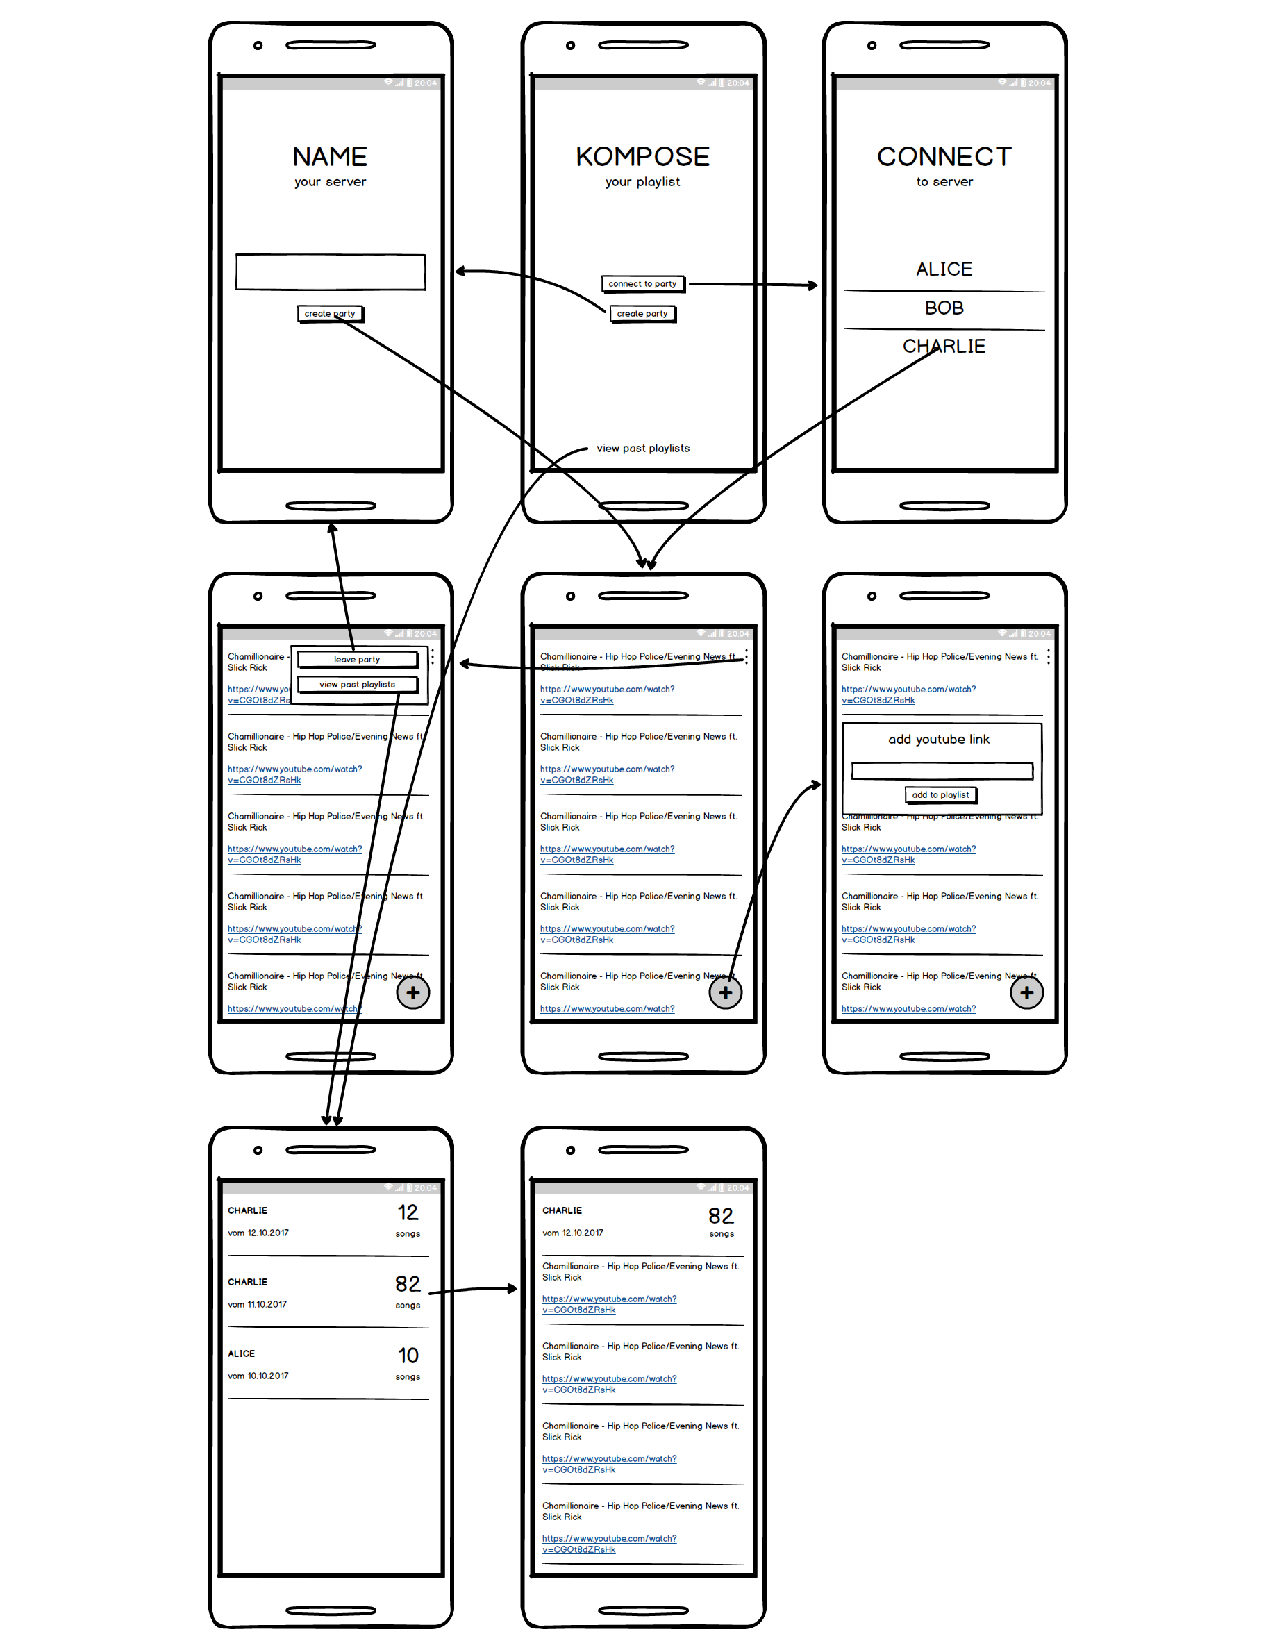
\includegraphics[width=\textwidth]{../design/mockups.pdf}
    \caption{User interface mockup (created with \cite{balsamiq})}
\end{figure*}

\end{document}
